\documentclass[a4paper,14pt, unknownkeysallowed]{extreport} 
\usepackage[hidelinks]{hyperref}
\usepackage[warn]{mathtext}
\usepackage[utf8]{inputenc}
\usepackage[T2A]{fontenc}
\usepackage[russian]{babel}
%\usepackage[14pt]{extsizes}
\usepackage{multirow}
\usepackage{listings}
\usepackage{graphicx}
\graphicspath{ {./img/} }
\usepackage{amsmath,amsfonts,amssymb,amsthm,mathtools} 
\usepackage{titlesec}
\usepackage{geometry}
\usepackage{amsmath}
\usepackage{caption}
\usepackage{subcaption}
\usepackage{graphicx}
\usepackage{lipsum}

\usepackage{pgfplots} % графики

% \usepgfplotslibrary{external} % кэширование графиков
% \tikzexternalize

\frenchspacing
\usepackage{indentfirst} % Красная строка

\usepackage{setspace}
\onehalfspacing % Полуторный интервал

\DeclareSymbolFont{T2Aletters}{T2A}{cmr}{m}{it} %Курсив кириллицы в формулах

\lstset{ %
basicstyle=\small\sffamily, % размер и начертание шрифта для подсветки кода
numbers=left,               % где поставить нумерацию строк (слева\справа)
numberstyle=\tiny,           % размер шрифта для номеров строк
stepnumber=1,                   % размер шага между двумя номерами строк
numbersep=5pt,                % как далеко отстоят номера строк от подсвечиваемого кода
showspaces=false,            % показывать или нет пробелы специальными отступами
showstringspaces=false,      % показывать или нет пробелы в строках
showtabs=false,             % показывать или нет табуляцию в строках
frame=single,              % рисовать рамку вокруг кода
tabsize=2,                 % размер табуляции по умолчанию равен 2 пробелам
captionpos=t,              % позиция заголовка вверху [t] или внизу [b] 
breaklines=true,           % автоматически переносить строки (да\нет)
breakatwhitespace=false, % переносить строки только если есть пробел
escapeinside={\#*}{*)}   % если нужно добавить комментарии в коде
}

\geometry{pdftex, left = 3cm, right = 10mm, top = 2cm, bottom = 2cm}

% Для измененных титулов глав:
\usepackage{titlesec, blindtext, color} % подключаем нужные пакеты
\definecolor{gray75}{gray}{0.75} % определяем цвет
\newcommand{\hsp}{\hspace{20pt}} % длина линии в 20pt

% caption for tables at top
\usepackage{float}
\floatstyle{plaintop}
\restylefloat{table}

\titleformat{\chapter}[hang]{\Huge\bfseries}{\thechapter\hsp\textcolor{gray75}{}\hsp}{0pt}{\Huge\bfseries}


\title{Lab 01 report}
\author{Kirill}

\date{\today}

\begin{document}
\thispagestyle{empty}

\noindent \begin{minipage}{0.15\textwidth}
	
\includegraphics[width=\linewidth]{b_logo}
\end{minipage}
\noindent\begin{minipage}{0.85\textwidth}\centering
	\textbf{Министерство науки и высшего образования Российской Федерации}\\
	\textbf{Федеральное государственное бюджетное образовательное учреждение высшего образования}\\
	\textbf{«Московский государственный технический университет имени Н.Э.~Баумана}\\
	\textbf{(национальный исследовательский университет)»}\\
	\textbf{(МГТУ им. Н.Э.~Баумана)}
\end{minipage}

\noindent\rule{16cm}{3pt}
\newline\newline
\noindent ФАКУЛЬТЕТ $\underline{\text{«Информатика и системы управления»}}$ \newline\newline
\noindent КАФЕДРА $\underline{\text{«Программное обеспечение ЭВМ и информационные технологии»}}$\newline\newline


\begin{center}
	\noindent\begin{minipage}{1.3\textwidth}\centering
	\Large\textbf{   ~~~ Лабораторная работа №3}\newline
	\textbf{по дисциплине "Анализ Алгоритмов"}\newline\newline\newline
	\end{minipage}
\end{center}

\noindent\textbf{Тема} $\underline{\text{Алгоритмы сортировки}}$\newline\newline
\noindent\textbf{Студент} $\underline{\text{Рядинский К. В.}}$\newline\newline
\noindent\textbf{Группа} $\underline{\text{ИУ7-53Б}}$\newline\newline
\noindent\textbf{Преподаватель} $\underline{\text{Волкова Л. Л.}}$\newline

\begin{center}
	\mbox{}
	\vfill
	Москва
\end{center}

\begin{center}
	\the\year ~г.
\end{center}
\clearpage


\tableofcontents
\newpage

\chapter*{Введение}
\addcontentsline{toc}{chapter}{Введение}


Целью данной лабораторной работы является изучить и реализовать алгоритмы сортировки, оценить их трудоемкость.

Алгоритмы сортировки имеют широкое практическое применение. Сортировки используются в большом спектре задач, включая обработку коммерческих, сейсмических, космических данных. Часто сортировка является просто вспомогательной операцией для упорядочивания данных, упрощения последующих алгебраических действий над данными.


Сортировка применяется во многих областях программирования, например, базы данных или математические программы. Упорядоченные объекты содержатся в телефонных книгах, ведомостях налогов, в библиотеках, в оглавлениях, в словарях.

Во многих вычислительных системах на сортировку уходит больше половины машинного времени. Исходя из этого, можно заключить, что либо сортировка имеет много важных применений, либо ею часто пользуются без нужды, либо применяются в основном неэффективные алгоритмы сортировки.

В настоящее время, в связи с экспоненциально возросшими объемами данных, вопрос эффективной сортировки данных снова стал актуальным. В настоящее время в сети Интернет можно найти результаты производительности алгоритмов сортировки для ряда ведущих центров данных.
При этом используются различные критерии оценки эффективности. 

Задачи лабораторной работы:

\begin{enumerate}
    \item Рассмотреть и изучить сортировки пузырьком, вставками и выбором.
    \item Реализовать каждую из этих сортировок.
    \item Расчитать их трудоемкость.
    \item Сравнить их временные характеристики экспериментально.
    \item На основании проделанной работы сделать выводы.
\end{enumerate}

\chapter{Аналитическая часть}
В данной главе будут рассмотрены алгоритмы сортировки.

\section{Сортировка пузырьком}


Алгоритм состоит из повторяющихся проходов по сортируемому массиву. За каждый проход элементы последовательно сравниваются попарно и, если порядок в паре неверный (возрастание, в случае сортировки по убыванию, и наоборот), выполняется обмен элементов. Проходы по массиву повторяются $N - 1$ раз, но есть модифицированная версия, где если окажется, что обмены больше не нужны, значит проходы прекращаются. При каждом проходе алгоритма по внутреннему циклу очередной наибольший элемент массива ставится на свое место в конце массива рядом с предыдущим «наибольшим элементом», а наименьший элемент массива перемещается на одну позицию к началу массива.

\section{Сортировка вставками}

Сортировка вставками — алгоритм сортировки, в котором элементы входной последовательности просматриваются по одному, и каждый новый поступивший элемент размещается в подходящее место среди ранее упорядоченных элементов.


В начальный момент отсортированная последовательность пуста. На каждом шаге алгоритма выбирается один из элементов входных данных и помещается на нужную позицию в уже отсортированной последовательности до тех пор, пока набор входных данных не будет исчерпан. В любой момент времени в отсортированной последовательности элементы удовлетворяют требованиям к выходным данным алгоритма.

\section{Сортировка выбором}

Шаги алгоритмы:

\begin{enumerate}
    \item Находится номер минимального значения в текущем списке.
    \item Производится обмен этого значения со значением первой неотсортированной позиции (обмен не нужен, если минимальный элемент уже находится на данной позиции).
    \item Сортируется хвост списка, исключиая при этом из рассмотрения уже отсортированные элементы.
\end{enumerate}

Для реализации устойчивости алгоритма необходимо в пункте 2. минимальный элемент непосредственно вставлять в первую неотсортированную позицию, не меняя порядок остальных элементов.

\section*{Вывод}

В данной работе стоит задача реализации 3 алгоритмов сортировки, а именно: пузырьком, вставками и выбором. Необходимо оценить трудоем- кость алгоритмов и проверить ее экспериментально.

\chapter{Конструкторская часть}

В данном разделе будут представлены схемы алгоритмов и рассчитана их трудоемкость.

\section{Трудоемкость алгоритмов}

\subsection{Модель вычислений}

Для последующего вычисления трудоемкости необходимо ввести модель вычислений.

\begin{enumerate}
    \item $+, -, /, \%, =, \neq, <, >, \leq, \geq, [ ], *, ++$ ~---~ трудоемкость 1.
    \item Трудоемкость оператора выбора \textit{if} условие \textit{then A else B} рассчитывается, как: 
    
    \begin{equation}
        f_{if} = f_{условия} + \begin{cases}
                                f_A & \quad \text{если условие выполняется,} \\
                                f_B & \quad \text{иначе}.
                                \end{cases}
    \end{equation}

    \item Трудоемкость цикла расчитывается, как:
    \begin{equation}
        f_{for} = f_{инициализации} + f_{сравнения} + N(f_{тела} + f_{инициализации} + f_{сравнения}).
    \end{equation}

    \item Трудоемкость вызова функции равна 0.
\end{enumerate}

\subsection{Расчет трудоемкости}

\subsubsection{Вычисление трудоёмкости алгоритма сортировки пузырьком}

\textbf{Лучший случай}: массив отсортирован, следовательно не произошло ни одного обмена.

Трудоемкость:

\begin{equation}
    T(N) = 2 + \frac{N \cdot (N - 1)}{2}\cdot 3 = 1.5N^2 - 1.5N + 2
\end{equation}

\textbf{Худший случай}: массив отсортирован в обратном порядке, в каждом случае происходил обмен.

Трудоемкость:

\begin{equation}
    T(N) = 2 + \frac{N \cdot (N - 1)}{2}\cdot 8 = 4N^2 - 4N + 2
\end{equation}

\subsubsection{Вычисление трудоёмкости алгоритма сортировки вставками}

\textbf{Лучший случай}: массив отсортирован, все внутренние циклы состоят всего из одной итерации.

Трудоемкость:

\begin{equation}
    T(N) = 2 + 6N
\end{equation}

\textbf{Худший случай}: массив отсортирован в обратном порядке. Каждый новый элемент сравнивается со всеми в отсортированной последовательности. Все внутренние циклы будут состоять из j итераций.

Трудоемкость.

\begin{equation}
    T(N) = \frac{N \cdot (N - 1)}{2} \cdot 10 + N + 2 = 5N^2 - 4N + 2
\end{equation}

\subsubsection{Вычисление трудоёмкости алгоритма сортировки выбором}

\textbf{Лучший случай}: массив отсортирован.

Трудоемкость:

\begin{equation}
    T(N) = 2 + \frac{N \cdot (N - 1)}{2} \cdot 8 + 4N = 4N^2 + 2
\end{equation}

\textbf{Худший случай}: массив отсортирован в обратном порядке, в каждом случае происходил обмен.

Трудоемкость:

\begin{equation}
    T(N) = \frac{N \cdot (N - 1)}{2} \cdot 5 + 5 \cdot N + 3 = 2.5N^2 + 2.5N + 3
\end{equation}

\section{Схемы алгоритмов}

На рисунке \ref{fig:bubble} изображена схема реализации алгоритма соритровки методом пузырька.

На рисунке \ref{fig:insertion} изображена схема реализации алгоритма соритровки методом вставок.

На рисунке \ref{fig:selection} изображена схема реализации алгоритма соритровки методом выбора.

\begin{figure}[h]
	\centering
	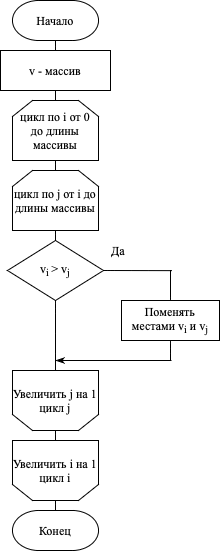
\includegraphics[scale=1]{bubble.png}
	\caption{Схема алгоритма сортировки пузырьком}
	\label{fig:bubble}
\end{figure}

\begin{figure}[h]
	\centering
	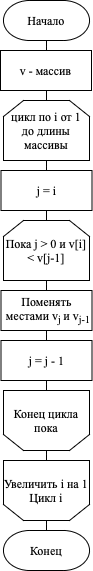
\includegraphics[scale=1]{insertion.png}
	\caption{Схема алгоритма сортировки вставками}
	\label{fig:insertion}
\end{figure}

\begin{figure}[h]
	\centering
	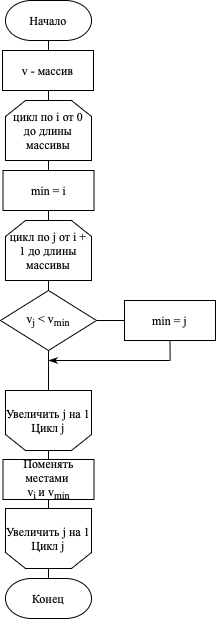
\includegraphics[scale=1]{selection.png}
	\caption{Схема алгоритма сортировки пузырьком}
	\label{fig:selection}
\end{figure}

\chapter{Технологическая часть}

В данном разделе приведены требования к программному обеспечению (далее ~--~ ПО), средства реализации и листинги кода

\section{Требования к ПО}

\textbf{Требования к вводу}
		
\begin{enumerate}
	\item На вход подается массив сравнимых элементов.
	\item На выходе --- отсортированный массив в заданном порядке;
\end{enumerate}

\section{Выбор языка программирования}
Для реализации программ я выбрал язык программирования Rust [1], так как этот язык предоставляет как низкоуровневые интерфейсы, так и высокоуровневые. Также он является таким же быстрым, как и С++, но более безопасен. Среда разработки Visual Studio Code.

\section{Листинги реализации алгоритма}

В листингах \ref{list:bubble} - \ref{list:selection} представлены реализации трех алгоритмов сортировки.

\begin{lstlisting}[label=list:bubble, caption=Функция сортировки массива методом пузырька]
pub fn bubble_sort<T: std::cmp::Ord>(v: &mut [T]) {
    for i in 0..v.len() {
        for j in i..v.len() {
            if v[i] > v[j] {
                v.swap(i, j);
            }
        }
    }
}
\end{lstlisting}

\begin{lstlisting}[label=list:insertion, caption=Функция сортировки массива методом вставок]
pub fn insertion_sort<T: std::cmp::Ord>(v: &mut [T]) {
    for i in 1..v.len() {
        let mut j = i;
        while j > 0 && v[j] < v[j - 1] {
            v.swap(j, j - 1);
            j = j - 1;
        }
    }
}
\end{lstlisting}

\begin{lstlisting}[label=list:selection, caption=Функция сортировки массива методом выбора]
pub fn selection_sort<T: std::cmp::Ord>(v: &mut [T]) {
    let mut min;
    for i in 0..v.len() {
        min = i;
        for j in (i + 1)..v.len() {
            if v[j] < v[min] {
                min = j;
            }
        }
        v.swap(i, min);
    }
}
\end{lstlisting}

\clearpage

\section{Тестирование}

Тестирование проводилось встроенной библиотекой модульного тестирования в систему сборки Cargo.

В таблице \ref{tab:tests} приведены результаты тестирования.

\begin{table}[h]
    \centering
    \begin{tabular}{|c|c|c|}
    \hline
    Вход       & Результат  & Ожидаемый результат \\ \hline
    1, 2, 3, 4 & 1, 2, 3, 4 & 1, 2, 3, 4          \\ \hline
    4, 3, 2, 1 & 1, 2, 3, 4 & 1, 2, 3, 4          \\ \hline
    1, 3, 2, 4 & 1, 2, 3, 4 & 1, 2, 3, 4          \\ \hline
    пустой     & пустой     & пустой              \\ \hline
    \end{tabular}
    \caption{Результаты функционального тестирования.}
    \label{tab:tests}
\end{table}


\section*{Вывод}

В данном разделе были представлены требования к программному обеспечению, выбор языка программирования, листинги реализаций алгоритмов и результаты тестирования.

\chapter{Исследовательская часть}

В данном разделе будут представлены замеры времени работы реализаций алгоритмов.

\section{Сравнительный анализ на основе замеров времени работы алгоритмов}
	
	Был проведен замер времени работы каждого из алгоритмов с помощью библиотеки Criterion [3]. Эта библиотека замеряет процессорное время выполнения функции и усредняет его.

    \begin{table}[]
        \centering
        \begin{tabular}{|c|c|c|c|}
        \hline
        Размер массива & Пузырек  & Вставки  & Выбором  \\ \hline
        10             & 5,50E-08 & 3,02E-08 & 6,20E-08 \\ \hline
        100            & 2,18E-06 & 1,07E-07 & 7,16E-06 \\ \hline
        500            & 4,44E-05 & 3,83E-07 & 2,24E-04 \\ \hline
        1000           & 1,69E-04 & 7,57E-07 & 9,34E-04 \\ \hline
        \end{tabular}
        \caption{Результаты времени выполнения алгоритмов сортировок на отсортированном массиве (в секундах)}
        \label{tab:sorted_bench}
    \end{table}

    \begin{figure}[h]
        \centering
    \begin{tikzpicture}
        \begin{axis}[
            xlabel={Количество элементов в массиве},
            ylabel={Время (в секундах)},
            width=8cm,
            height=8cm,
            legend pos=north west,
            ymajorgrids=true,
            grid style=dashed,
        ]

        \addplot[
            color=blue,
            mark=square,
            ]
            coordinates {
                (10, 5.50e-8)(100, 2.18e-6)(500, 4.44e-5)(1000, 1.69e-4)
            };
            \addlegendentry{Пузырек}
        \addplot[
            color=red,
            mark=triangle,
            ]
            coordinates {
                (10, 3.02e-8)(100, 1.07e-7)(500, 3.82e-7)(1000, 7.57e-7)
            };
            \addlegendentry{Вставки}
        \addplot[
            color=black,
            mark=star,
            ]
            coordinates {
                (10, 6.20e-8)(100, 7.16e-6)(500, 2.24e-4)(1000, 9.34e-4)
            };
            \addlegendentry{Выбор}
    
    \end{axis}
    \end{tikzpicture}
    \caption{График времени выполнения алгоритмов при отсортированном массиве}
    \end{figure}

    \begin{table}[]
        \centering
        \begin{tabular}{|c|c|c|c|}
        \hline
        Размер массива & Пузырек  & Вставки  & Выбором  \\ \hline
        10             & 6,80E-08 & 8,14E-08 & 1,22E-07 \\ \hline
        100            & 2,54E-06 & 8,00E-06 & 7,55E-06 \\ \hline
        500            & 5,66E-05 & 2,01E-04 & 2,27E-04 \\ \hline
        1000           & 2,16E-04 & 8,25E-04 & 9,33E-04 \\ \hline
        \end{tabular}
        \caption{Результаты времени выполнения алгоритмов сортировок на отсортированном в обратном порядке массиве (в секундах)}
        \label{tab:unsorted_bench}
    \end{table}

    \begin{figure}[h]
    \centering
    \begin{tikzpicture}
        \begin{axis}[
            xlabel={Количество элементов в массиве},
            ylabel={Время (в секундах)},
            width=8cm,
            height=8cm,
            legend pos=north west,
            ymajorgrids=true,
            grid style=dashed,
        ]

        \addplot[
            color=blue,
            mark=square,
            ]
            coordinates {
                (10, 6.80e-08)(100, 2.54e-06)(500, 5.66e-05)(1000, 2.16e-04)
            };
            \addlegendentry{Пузырек}
        \addplot[
            color=red,
            mark=triangle,
            ]
            coordinates {
                (10, 8.14e-08)(100, 8.00e-06)(500, 2.01e-04)(1000, 8.25e-04)
            };
            \addlegendentry{Вставки}
        \addplot[
            color=black,
            mark=star,
            ]
            coordinates {
                (10, 1.22e-07)(100, 7.55e-06)(500, 2.27e-04)(1000, 9.33e-04)
            };
            \addlegendentry{Выбор}
    
    \end{axis}
    \end{tikzpicture}
    \caption{График времени выполнения алгоритмов при отсортированном в обратном порядке массиве}
    \end{figure}

    \begin{table}[]
        \centering
        \begin{tabular}{|c|c|c|c|}
        \hline
        Размер массива & Пузырек  & Вставки  & Выбором  \\ \hline
        100            & 2,91E-06 & 3,75E-06 & 8,72E-06 \\ \hline
        1000           & 3,32E-04 & 4,11E-04 & 9,48E-04 \\ \hline
        2500           & 2,02E-03 & 2,55E-03 & 5,99E-03 \\ \hline
        5000           & 8,27E-03 & 1,02E-02 & 2,43E-02 \\ \hline
        \end{tabular}
        \caption{Результаты времени выполнения алгоритмов сортировок на случайном массиве (в секундах)}
        \label{tab:rand_bench}
    \end{table}

    \begin{figure}[h]
        \centering
    \begin{tikzpicture}
        \begin{axis}[
            xlabel={Количество элементов в массиве},
            ylabel={Время (в секундах)},
            width=10cm,
            height=8cm,
            legend pos=north west,
            ymajorgrids=true,
            grid style=dashed,
        ]

        \addplot[
            color=blue,
            mark=square,
            ]
            coordinates {
                (100, 2.91e-06)(1000, 3.32e-04)(2500, 2.02e-03)(5000, 8.27e-03)
            };
            \addlegendentry{Пузырек}
        \addplot[
            color=red,
            mark=triangle,
            ]
            coordinates {
                (100, 3.75e-06)(1000, 4.11e-04)(2500, 2.55e-03)(5000, 1.02e-02)
            };
            \addlegendentry{Вставки}
        \addplot[
            color=black,
            mark=star,
            ]
            coordinates {
                (100, 8.72e-06)(1000, 9.48e-04)(2500, 5.99e-03)(5000, 2.43e-02)
            };
            \addlegendentry{Выбор}
    
    \end{axis}
    \end{tikzpicture}
    \caption{График времени выполнения алгоритмов при случайном массиве}
    \end{figure}

    \section*{Вывод}

    По результатам тестирования выявлено, что все рассматриваемые алгоритмы реализованы правильно. Самым быстрым алгоритмом при использовании случайного массива оказался алгоритм сортировки методом пузырька. Метод выбора является самый медленным на случайном наборе данных.

    \chapter*{Заключение}

    В рамках данной лабораторной работы:

    \begin{itemize}
        \item были изучены и реализованы три алгоритма сортировки: методом пузырька, вставок и выбором;
        \item был проведен сравнительный анализ трудоемкости алгоритмов на основе теоретических расчетов и выбранной модели вычислений;
        \item был проведен сравнительный анализ алгоритмов на основе экспериментальных данных;
    \end{itemize}

    Экспериментально были установлены различия в производительности различных алгоритмов сортировки. Для массивов длины 5000, заполненной случайными данными, метод пузырька быстрее вставок и выбора.
\end{document}
